\section{Background}

In April 2019, LSST DM began a proof of concept project with the AWS and HTCondor teams to explore whether a cloud deployment of the Data Release Production (DRP) is feasible. The execution plan of the project is described in DMTN-114.  In this document we report the results.



\section{Approaches and Strategies}

In executing this PoC we focused on the goal of being able to demonstrate the data processing on the AWS cloud and kept the following strategies in mind.



\begin{enumerate}
\item
Progress in phases.
\end{enumerate}


\section{Architecture Design}

The system design in the end of the PoC is as in the diagram in Figure~\ref{fig:arch}.

\begin{figure}
  \centering
  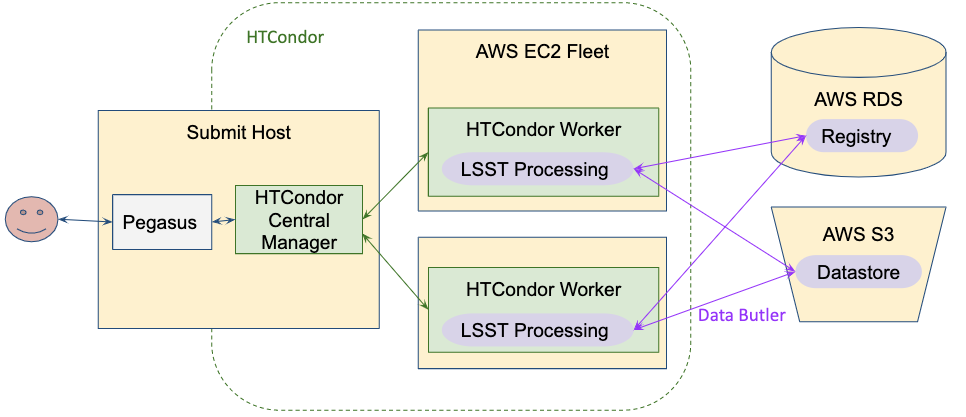
\includegraphics[width=\textwidth]{figures/arch}
  \label{fig:arch}
  \caption{architecture design}
\end{figure}

\subsection{Alternative architecture designs were also discussed in the PoC}


\section{Data Butler Repository on the AWS Cloud}

In the PoC we implemented new features to enable a cloud-based Data Butler.

S3 Datastore
From POSIX filesystem to object store backend.

RDS Registry
PostgreSQL


\section{Results of the tract-sized runs}
